\documentclass[11pt]{article}
\usepackage[margin=1.1in]{geometry}
\usepackage{booktabs}
\usepackage{graphicx}
\usepackage{amsmath}
\usepackage[hidelinks]{hyperref}
\usepackage{microtype}
\usepackage{xcolor}
\usepackage[section]{placeins}

\hyphenation{un-at-trib-ut-able}

\newcommand{\iaf}{\textsc{iaf}}
\newcommand{\eci}{\textsc{eci}}

\title{Economic Integrity in Production LLM Pipelines:\\
Measuring Attempt Amplification, Discarded Reasoning,\\
and Retry Cost}

\author{Sean Halverson\\VuduVations \textperiodcentered{} \texttt{vuduvations.io}\\\texttt{hello@vuduvations.io}}
\date{August 2026 \quad (preprint v0.2)}

\begin{document}
\maketitle

\begin{center}
\small\textit{Patent pending. One or more U.S. provisional patent applications have been filed covering aspects of the systems and methods described herein.}
\end{center}

\begin{abstract}
Model pricing pages quote cost per token. Production pipelines pay per
\emph{attempt}. When a pipeline retries empty replies, when its validation
layers re-ask failed roles, and when reasoning models bill thinking tokens
for outputs they never emit, the invoice decouples from the scoreboard.
In a companion reliability study we reported this decoupling as an
instrumentation gap: attempts were not instrumented, so attempt
denominators were unavailable and starvation could only be counted from
run logs. This paper closes that gap. We add a per-attempt economic
ledger at the HTTP boundary of a production analysis pipeline --- one
record per physical model call, carrying token counts including reasoning
and prompt-cache splits, budgets, lever state, layer, outcome, and
latency --- and re-run a four-cell budget/retry ablation
($n{=}10$ repetitions per cell, one provider, one night) with the ledger
armed. We define two metrics over the ledger: the \emph{Inference
Amplification Factor} (\iaf{}), physical attempts per logical job, and the
\emph{Economic Contamination Index} (\eci{}), total spend over spend on
attempts whose output was actually used. All four cells were
scoreboard-equivalent --- answer-key means of 46.8--47.4 of 48 checks
and 9--10 of 10 execution-clean or recovered-clean repetitions;
underneath, the attempt machinery differed by up to a factor of $1.7$.
Proactive budget headroom \emph{measures} as prevention: one starved
first attempt in 127 agent-layer jobs, and --- with the retry disabled,
so no recovery could hide it --- no amplification at either recovery
ring (\iaf{} $=1.000$ by direct enumeration). Retry-based recovery
reaches an equivalent scoreboard with \iaf{} up to $1.70$ and \eci{} up
to $1.96$ in the
adversarial validation layer: in the worst cell, 48.9\% of that layer's
spend bought attempts whose output was discarded --- and every discarded
output token in the study was a reasoning token, the spend category no
scoreboard sees. Rescue effectiveness was also non-stationary: a
same-budget re-ask recovered roughly 19 of 20 starved jobs one night and
5 of 16 two nights later under an identical configuration, so retry-based
cost forecasts inherit a volatility that prevention-based forecasts do
not. Across the study, 9.6\% of ledger-computed spend bought discarded
attempts. A retry repairs the answer. It does not erase the first
invoice.
\end{abstract}

\section{Introduction}

Benchmark papers report accuracy per task. Pricing pages report dollars
per million tokens. Between the two sits an object neither one measures:
the \emph{attempt}. A production pipeline that values availability will
retry an empty reply, re-ask a failed validation role, and salvage what
it can; each of those recovery actions is a fresh, billed model call
whose predecessor's cost is already sunk. When the model family is a
reasoning model, the sunk cost is worse than it looks: an attempt that
exhausts its completion budget on chain-of-thought and emits zero
visible output still bills its reasoning tokens at the output
rate~\cite{openaireasoning,deepseekdocs}. The scoreboard records one
answer. The invoice records every attempt. Nothing in the standard
reporting stack reconciles the two.

Our companion reliability study~\cite{reliability} documented the
epistemic half of this problem: a fallback-enabled pipeline can produce
near-perfect benchmark scores while the probabilistic component under
test did not produce them, and run-level \emph{degradation accounting}
is required to tell the difference. That paper counted starvation
\emph{events} from run logs and was explicit about its boundary:
attempts were not instrumented, so it declined attempt denominators and
reported counts, not rates. The present paper is the economic half. We
instrument the attempt itself and ask what the recovery machinery
\emph{costs} --- not in the aggregate-bill sense, but attributed per
attempt, per layer, and per outcome.

The contributions are:

\begin{enumerate}
\item \textbf{An attempt-level economic ledger} (Section~\ref{sec:instrumentation}):
one JSONL record per physical HTTP model call, written inside the
pipeline's portable client below all metering wrappers, carrying input,
output, and reasoning token counts, prompt-cache hit/miss splits,
requested and sent budgets, intervention-lever state, pipeline layer,
attempt number, outcome, and latency. The hook is armed by an
environment variable and is a strict no-op otherwise; the pipeline's
legacy per-run token counters are deliberately unchanged, so the
ledger-versus-legacy delta is itself a measurement of what conventional
metering misses.
\item \textbf{Two metrics with measured denominators}
(Section~\ref{sec:framework}): the Inference Amplification Factor
(\iaf{}), physical attempts per logical job, computed per pipeline layer
and never pooled across layers; and the Economic Contamination Index
(\eci{}), total spend over spend on used attempts, where \emph{used} is
defined exactly (the final attempt of a logical job, when non-empty).
\item \textbf{A measured four-cell ablation} (Sections~\ref{sec:design}--\ref{sec:results}):
the companion paper's budget/retry ablation re-run with the ledger armed
($n{=}10$ per cell, DeepSeek v4-pro direct, 2026-08-10/11). Every cell
was scoreboard-equivalent (answer-key means 46.8--47.4 of 48; 9--10 of
10 execution-clean or recovered-clean repetitions); the cells' \iaf{}
and \eci{} separated cleanly, and in the direction the companion
paper's event counts predicted.
\item \textbf{Three economic findings}: prevention is measurable by
enumeration --- a counted starvation residual with no hidden recovery
amplification --- rather than inferable from absence of log lines
(Section~\ref{sec:prevention}); the adversarial validation layer, whose
role calls run on small completion budgets, was the study's dominant
amplifier, with up to half its spend discarded
(Section~\ref{sec:amplifier}); and rescue rates moved by a factor of
about three across two nights under identical configuration, which
bounds how retry-heavy architectures can be cost-forecast
(Section~\ref{sec:nonstationarity}).
\end{enumerate}

We state the scope plainly, as in the companion study: this is a
measurement-method case study on one production pipeline, one provider,
one night per cell, $n{=}10$ per cell. The numbers are counts and
dollars with denominators we measured, not rates we expect to
generalize. What we believe generalizes is the instrument and the two
metrics.

\section{The Hidden Denominator Problem}\label{sec:hidden}

Three mechanisms make the attempt invisible to conventional accounting.

\textbf{Retries rebind the response.} A recovery path that retries an
empty reply typically overwrites the failed response object with the
successful one; whatever token metering reads the response afterward
meters only the survivor. Our own pipeline had exactly this seam: the
portable client's empty-reply retry rebound the response variable, so
the first attempt's tokens --- a starved attempt bills its entire
reasoning budget --- were counted by nothing. The pipeline's per-run
counters, and every figure derived from them, silently reported the
cost of the attempts that \emph{worked}.

\textbf{Reasoning tokens are invisible output.} On reasoning-mode
models, chain-of-thought is billed at the output rate but is not part
of the visible completion~\cite{openaireasoning,deepseekdocs}. A
starved attempt --- one that spends its whole completion budget
thinking and emits nothing --- therefore produces a bill with no
corresponding artifact anywhere in the application. In this study,
65.1\% of all billed output tokens were reasoning tokens, and, within
one token of exactly, \emph{100\% of discarded output tokens were
reasoning tokens}: the attempts the pipeline threw away consisted
entirely of thinking no one ever saw.

\textbf{Layered recovery multiplies callers.} Production pipelines
recover at more than one level. In ours, the portable client retries an
empty reply once; above it, the adversarial validation layer's
orchestrator can re-ask a failed role as a fresh call. Each ring of
recovery bills separately, and an aggregate invoice cannot attribute
spend to rings. Only an attempt-level record with a logical-job
identity can.

The result is a denominator problem. ``Cost per task'' has a measured
numerator (the bill) and an assumed denominator (one attempt per task).
The companion study showed the assumption failing at rates up to 96
starvation events per ten repetitions~\cite{reliability} --- but could
not price it, because the failed attempts were not instrumented. The
remainder of this paper is the pricing.

\section{The Economic Integrity Framework}\label{sec:framework}

\textbf{Three layers of integrity.} A production result can be
interrogated at three depths. \emph{Capability integrity}: did the
answer satisfy the task? This is what the benchmark's 48-check answer
key grades. \emph{Execution integrity}: did the intended model path
produce it? This is the companion paper's degradation
accounting~\cite{reliability} --- fallbacks, salvages, and retries that
leave the answer intact while changing what produced it.
\emph{Economic integrity}: how many paid physical attempts stood behind
the accepted output? Each layer can pass while the next fails silently:
a correct answer can come from a fallback, and a fallback-free run can
have paid for twice the attempts its architecture diagram shows. This
paper supplies the third layer's instrument and metrics; the four cells
of Section~\ref{sec:results} are precisely a set of configurations that
tie on the first layer, mostly tie on the second, and separate on the
third.

We define the metrics over an attempt ledger: a set of records, one per
physical model call, each carrying a logical-job identity, an attempt
number within that job, token counts, and an outcome.

\textbf{Logical job.} One unit of work the pipeline intended: one agent
completion, one validation-role completion. A logical job is identified
by its calling site and a per-run sequence number, so two calls from
the same site are distinct jobs, and a retry of one call is the same
job.

\textbf{Physical attempt.} One HTTP round trip that was billed (or
errored). A logical job has one or more physical attempts.

\textbf{Inference Amplification Factor.} For a set of logical jobs $J$
with physical attempts $A$,
\[
\iaf{} = \frac{|A|}{|J|}.
\]
$\iaf{} = 1$ means every job succeeded on its first attempt; $\iaf{} =
1.5$ means half again as many calls were made as the architecture
diagram shows. We compute \iaf{} \emph{per pipeline layer} (primary
agents versus the adversarial validation layer) and never pool layers:
the layers run different budgets, different prompt shapes, and
different recovery policies, and a pooled figure would average away
exactly the structure the metric exists to expose.

\textbf{Used attempt.} The final attempt of a logical job, when its
content is non-empty. Every other attempt --- an empty attempt that was
retried, or a final attempt that was itself empty --- was paid for and
discarded. This definition is deliberately conservative in one known
way: the pipeline has salvage paths that can extract partial value from
a malformed reply, and the ledger classifies such a reply by emptiness,
not by downstream salvage. \eci{} as computed here is therefore a mild
upper bound on contamination.

\textbf{Economic Contamination Index.} For a layer with total attempt
spend $C_{\text{total}}$ and spend on used attempts $C_{\text{used}}$,
\[
\eci{} = \frac{C_{\text{total}}}{C_{\text{used}}}.
\]
$\eci{} = 1$ means every dollar bought output that was used; $\eci{} =
2$ means half the spend bought discarded attempts. \eci{} is the
economic analogue of the companion paper's fallback contamination: there,
the scoreboard was contaminated by answers the model under test did not
produce; here, the invoice is contaminated by attempts the application
never used.

Both metrics have \emph{measured} denominators: every physical attempt
in this study is a ledger row, including attempts that errored at the
transport layer. The companion paper's caveat --- ``attempts were not
instrumented'' --- does not apply to these runs.

\section{Instrumentation}\label{sec:instrumentation}

\textbf{Placement.} The ledger hook lives inside the pipeline's
portable LLM client, immediately around each transport-level completion
call --- below the benchmark's metering wrapper and below the client's
own retry logic. Placement matters twice over. First, it sits under the
response-rebinding seam described in Section~\ref{sec:hidden}, so the
starved first attempt that legacy metering loses is a first-class row.
Second, the adversarial validation layer's role calls route through the
same injected client in this configuration, so chamber traffic is
captured by the same hook with no second instrument.

\textbf{Record schema.} Each row carries: timestamp; experiment cell
and repetition; logical job id (calling agent name plus per-run
sequence); layer (\texttt{agent} or \texttt{debate}, derived from the
calling site, never pooled downstream); attempt number; requested and
sent completion budgets; the state of the three intervention levers;
input, output, and \emph{reasoning} token counts from the provider's
usage object; prompt-cache hit and miss token splits; finish reason;
serving identity where exposed; a content-emptiness flag; outcome
(\texttt{ok}, \texttt{empty}, or \texttt{error}); and wall-clock
latency. Rows are appended to a JSONL file named by an environment
variable; when the variable is unset the hook is a no-op, and the
instrumented client shipped to production with the hook dormant.
Ledger writes never fail a run: an unwritable ledger degrades to a
warning.

\textbf{The nested retry topology.} The pipeline recovers at two rings,
and the ledger records them differently, on purpose. The portable
client's own empty-reply retry is the \emph{same logical job}, attempt
number 2. The validation orchestrator's re-ask of a failed role is a
\emph{new logical job}: it arrives at the client as a fresh call from
the same calling site and takes the next sequence number. This is not a
limitation but a feature of the identity design: ring membership is
recoverable from the ledger (attempt numbers expose the inner ring;
job-count inflation at a fixed calling-site population exposes the
outer ring), and Section~\ref{sec:amplifier} uses exactly this
signature --- 193 debate-layer logical jobs in the cell whose inner
retries mostly failed, against 110--119 in the others --- to observe
the outer ring engaging when the inner ring fails.

\textbf{Legacy counters unchanged.} The client's pre-existing token
counters, which meter only the returned attempt, were deliberately left
untouched, for two reasons. They preserve comparability with the
companion paper's published figures. And the delta between ledger and
legacy totals is itself the headline measurement: it is precisely the
paid-but-discarded spend that conventional metering cannot see.

\textbf{Pricing basis.} Dollar figures computed from the ledger use the
provider's undiscounted direct list rates (\$0.435 input, \$0.87 output
per million tokens~\cite{deepseekdocs}), with cache-hit input tokens
priced at the full input rate. Ledger-computed dollars are therefore
upper bounds; hit/miss splits are recorded per attempt for
re-pricing. Section~\ref{sec:accounting} reconciles this basis against
the account-billed total.

\section{Experimental Design}\label{sec:design}

The workload is the companion study's fixed benchmark: four analysis
protocols over a frozen fictional corpus, graded by a 48-check answer
key, roughly 12--13 agent-layer completions and a multi-role
adversarial validation pass per repetition~\cite{reliability}. The
model is DeepSeek v4-pro on the direct first-party channel, the same
model and channel as the companion paper's post-fix runs. The
manipulated factors are the same two mechanisms as the companion
ablation, crossed into four cells:

\begin{table}[!htb]
\centering\small
\begin{tabular}{lll}
\toprule
Cell & Proactive headroom & Empty-reply retry \\
\midrule
\emph{reactive} & off & on, retry adds headroom \\
\emph{proactive} & on & off \\
\emph{pure retry} & off & on, retry at unchanged budget \\
\emph{bundle} & on & on, retry adds headroom \\
\bottomrule
\end{tabular}
\caption{The four cells. \emph{Proactive headroom} raises completion
budgets before the first attempt; the \emph{reactive} and \emph{bundle}
retries add the same headroom only on the second attempt; the
\emph{pure retry} cell re-asks at the unchanged budget, isolating
re-sampling from budget relief. Cell configuration is applied by
process environment at launch; the run-of-record script clears all
levers between cells.}
\label{tab:cells}
\end{table}

Each cell ran $n{=}10$ repetitions (five launches of two repetitions
each, matching the companion run-of-record shape) on 2026-08-10/11,
with the ledger armed and a balance-floor guard between cells. Unlike
the companion ablation, whose cells were launched by hand, the entire
run is a committed script; the raw ledgers (one JSONL per cell), the
twenty per-launch result files, the analyzer, and the compiled report
are all committed alongside it (Section~\ref{sec:artifacts}).

One asymmetry with the companion paper must be stated up front: these
are \emph{new} runs on a \emph{different night}, not a re-analysis of
the companion cells. The companion ablation's agent-layer starvation
ran 96--102 events per no-headroom cell on 2026-08-09; tonight the same
configurations produced 12--16. Cross-night variance of this size is
itself one of the paper's findings
(Section~\ref{sec:nonstationarity}), and it is why every figure below
carries its own denominators and no figure is offered as a rate.

\section{Results}\label{sec:results}

Table~\ref{tab:main} is the study's central result. All four cells were
scoreboard-equivalent, in the two senses Table~\ref{tab:tiers} makes
precise. On capability, answer-key totals ran 468--474 of 480 checks
(cell means 46.8--47.4 of 48), and the differences do not order the
cells --- the only cell with 10 of 10 execution-clean-or-recovered
repetitions has the \emph{lowest} answer-key mean. On execution, every
cell produced 9--10 of 10 repetitions that were execution-clean or
recovered-clean. The attempt machinery underneath was not equivalent.

\begin{table}[!htb]
\centering\small
\setlength{\tabcolsep}{4.5pt}
\begin{tabular}{llrrrrrrrrrr}
\toprule
Cell & Layer & Jobs & Att. & \iaf{} & Starved & Rec. & Unrec. &
Total \$ & Used \$ & Disc.\ \$ & \eci{} \\
\midrule
reactive & agent & 126 & 137 & 1.087 & 12 & 11 & 1 & 0.643 & 0.628 & 0.015 & 1.023 \\
 & debate & 119 & 202 & \textbf{1.698} & 83 & 82 & 1 & 0.289 & 0.184 & 0.106 & 1.576 \\
\addlinespace
proactive & agent & 127 & 127 & \textbf{1.000} & 1 & 0 & 1 & 0.680 & 0.680 & 0.000 & 1.000 \\
 & debate & 119 & 119 & \textbf{1.000} & 1 & 0 & 1 & 0.190 & 0.190 & 0.001 & 1.003 \\
\addlinespace
pure retry & agent & 128 & 142 & 1.109 & 16 & 5 & 11 & 0.652 & 0.623 & 0.029 & 1.046 \\
 & debate & 193 & 281 & 1.456 & 88 & 19 & 69 & 0.380 & 0.194 & \textbf{0.186} & \textbf{1.957} \\
\addlinespace
bundle & agent & 124 & 126 & 1.016 & 2 & 2 & 0 & 0.689 & 0.670 & 0.020 & 1.029 \\
 & debate & 110 & 110 & \textbf{1.000} & 0 & 0 & 0 & 0.171 & 0.171 & 0.000 & 1.000 \\
\bottomrule
\end{tabular}
\caption{Measured attempt economics per cell and layer ($n{=}10$
repetitions per cell, DeepSeek v4-pro direct, 2026-08-10/11).
\emph{Jobs} are logical jobs, \emph{Att.} physical attempts,
\emph{Starved} first attempts returning empty, \emph{Rec.}/\emph{Unrec.}
starved jobs whose final attempt was non-empty/empty. Dollars are
ledger-computed at undiscounted list rates with cache-hit input at the
full input rate (upper bounds; Section~\ref{sec:accounting}). Layers
are never pooled. Agent-layer job counts exceed the ten graded agents
because summarizer and validator completions share the layer; the
outcome tiers in Table~\ref{tab:tiers} still grade on the ten-agent
basis of the companion paper. The proactive agent layer's single
starved job was a zero-token transport error, hence discarded spend of
\$0.000.}
\label{tab:main}
\end{table}

\begin{table}[!htb]
\centering\small
\setlength{\tabcolsep}{4.5pt}
\begin{tabular}{lccccr}
\toprule
Cell & Answer key (mean) & 1st-att.\ clean & Recovered clean & Degraded & Agent \$/rep \\
\midrule
reactive & 470/480 \ (47.0) & 0 & 9 & 1 & 0.064--0.067 \\
proactive & 474/480 \ (47.4) & 9 & 0 & 1 & 0.065--0.068 \\
pure retry & 472/480 \ (47.2) & 0 & 9 & 1 & 0.055--0.066 \\
bundle & 468/480 \ (46.8) & 8 & 2 & 0 & 0.067--0.078 \\
\bottomrule
\end{tabular}
\caption{Per-repetition scoreboards: answer-key totals (48-check
benchmark, ten repetitions per cell) beside execution tiers (ten-agent
grading basis joined to per-repetition ledger cost). The two are
distinct measurements and neither orders the cells: the bundle is the
only cell with zero degraded repetitions and also has the lowest
answer-key mean. Mean agent-layer cost per repetition is nearly flat
across cells and tiers at tonight's event rates: the economic
difference between the cells lives in Table~\ref{tab:main}'s debate
rows and in attempt-count variance, not in the per-repetition agent
bill.}
\label{tab:tiers}
\end{table}

\begin{figure}[!htb]
\centering
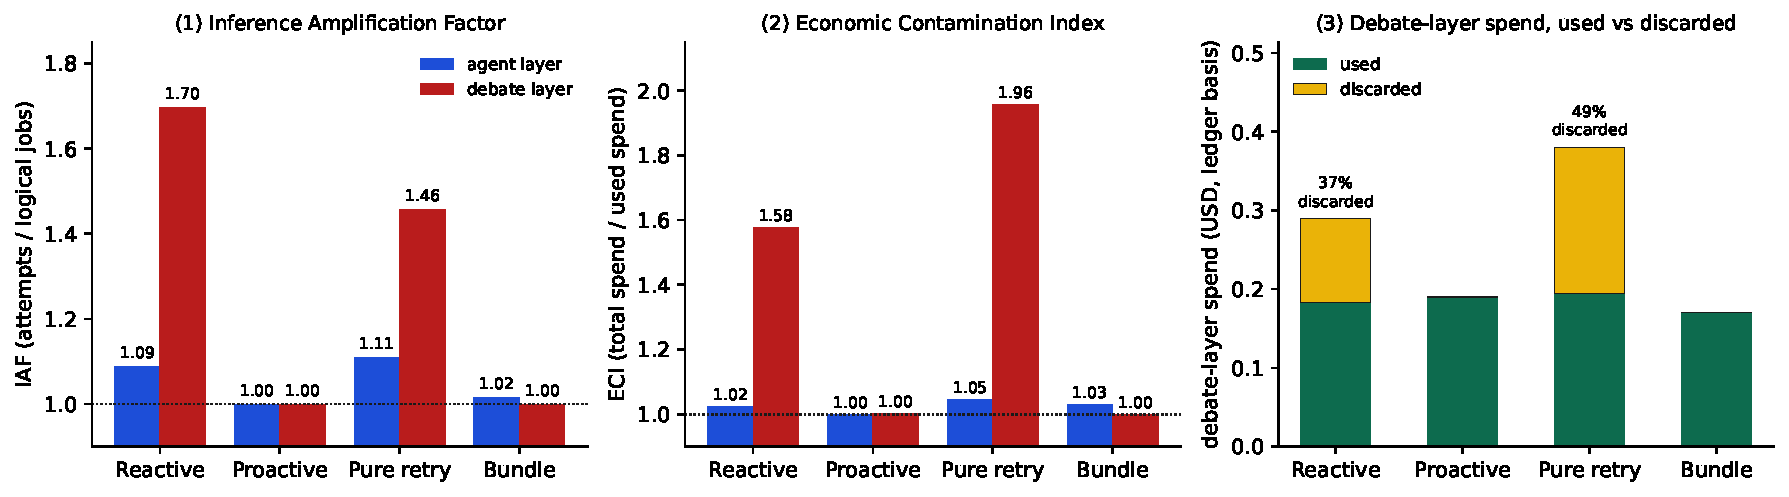
\includegraphics[width=\textwidth]{fig_econ.pdf}
\caption{The measured attempt economics of Table~\ref{tab:main}
($n{=}10$ repetitions per cell, DeepSeek v4-pro direct, 2026-08-10/11;
every value is read programmatically from the compiled report, none
transcribed). Panels 1 and 2 show \iaf{} and \eci{} per layer, never
pooled; the dotted line at $1.0$ is the no-amplification floor that
both proactive rows sit on. Panel 3 splits the adversarial validation
layer's ledger-computed spend into used and discarded dollars: the two
no-headroom cells discarded 37\% and 49\% of the layer's bill to reach
a scoreboard equivalent to the cells that discarded none.}
\label{fig:econ}
\end{figure}

Four observations organize the rest of the paper.

\textbf{(1) Scoreboard equivalence hid a $1.7\times$ attempt spread.}
The reactive cell's debate layer made 202 physical calls to complete
119 logical jobs (\iaf{} $=1.698$); the proactive cell's made 119 for
119. Both cells were scoreboard-equivalent (answer-key means 47.0 and
47.4; nine of ten repetitions clean or recovered). Nothing on either
scoreboard, and nothing in legacy returned-attempt metering, distinguishes them.

\textbf{(2) Discarded spend concentrates where budgets are tight.} The
adversarial validation layer runs its roles on small completion
budgets; without headroom it starved 83--88 times per cell and its
\eci{} reached 1.58--1.96. The agent layer, on generous budgets
tonight, held \eci{} at 1.02--1.05 everywhere. Across the whole study,
\$0.355 of \$3.694 ledger-computed spend --- 9.6\% --- bought attempts
whose output was discarded, and 82\% of that discarded spend was in the
debate layer.

\textbf{(3) Every discarded output token was a reasoning token.} Summed
over all cells and layers, discarded attempts billed 228{,}890 output
tokens, of which 228{,}889 were reasoning tokens (the one-token gap is
a provider rounding artifact). A starved attempt spends its entire
completion budget thinking and emits nothing; the entire discarded
bill was invisible thinking. Overall, 65.1\% of the study's billed
output tokens were reasoning tokens, so the spend category most
exposed to discard is also the largest one.

\textbf{(4) The ledger measured the outer recovery ring engaging.} The
pure-retry cell's debate layer shows 193 logical jobs against 110--119
in every other cell. Its inner retries mostly failed (19 of 88 starved
jobs recovered at the unchanged budget), and the failures surfaced to
the validation orchestrator, whose re-asks arrive as fresh logical
jobs (Section~\ref{sec:instrumentation}). The job-count inflation is
the outer ring's billing signature: recovery that fails at one ring
does not end the spending, it escalates it to the next ring's budget.

\section{Recovery Is Not Prevention, Priced}\label{sec:prevention}

The companion paper's ablation attributed \emph{prevention} of
first-attempt starvation to proactive headroom and characterized retry
as insurance~\cite{reliability}. The ledger now prices that
distinction, and closes a measurement blind spot in it.

\textbf{Prevention measures as a counted residual with no hidden
amplification.} One caveat first: in the proactive cell the client
retry is ablated, so inner-ring \iaf{} cannot exceed $1$ by
construction --- \iaf{} $=1.000$ is not, by itself, the evidence. The
evidence is three measured facts the ledger adds. First, the
starvation residual is enumerated, not inferred: 127 agent-layer jobs,
127 attempts, one empty reply (a zero-token transport error, a class
no completion budget can prevent); 119 debate-layer jobs, 119
attempts, one starved. The companion paper's ``zero starvation
events'' claim had rested on the absence of a retry log line --- a
line that \emph{cannot fire} in that cell, because the retry is the
thing ablated; absence of evidence from a disabled instrument is not
evidence of absence, and the ledger replaces that inference with
enumeration. Second, the outer recovery ring did not engage: the
validation orchestrator's re-asks register as extra logical jobs
(Section~\ref{sec:instrumentation}), and the debate-layer job count
sits at the baseline 119, not the 193 of the cell where inner
recovery failed. Third, the two residual empties went unrecovered ---
headroom without retry has no insurance, which is the bundle's
argument. The claim survives direct measurement --- as 1-in-127, not
zero, which is how such claims should be stated.

\textbf{Recovery reaches an equivalent scoreboard and pays for both
attempts.} The reactive cell's scoreboard was equivalent to
proactive's (nine of ten repetitions clean or recovered; answer-key
means 47.0 versus 47.4). To
get there its debate layer paid for 202 attempts against 119 jobs,
discarding \$0.106 of \$0.289 --- 36.5\% of that layer's bill --- while
the proactive cell's debate layer discarded \$0.0006. On tonight's calm
agent layer the per-repetition bills were nearly identical across
cells (Table~\ref{tab:tiers}); the economic difference between
recovery and prevention lived in the tight-budget layer and in
latency and variance, not in the agent-layer bill. On the companion
paper's night, when the agent layer starved 96--102 times per cell,
the same structural difference would have priced an order of magnitude
higher. That contrast is the forecasting point of
Section~\ref{sec:nonstationarity}: prevention's cost is stable by
construction (one attempt per job); recovery's cost is a random
variable.

\textbf{Retry still earns its place.} The bundle cell --- headroom plus
retry --- was the only cell with zero degraded repetitions, and its two
first-attempt agent starvations were both recovered by the retry at a
discarded cost of \$0.020. As in the companion study, the argument is not against retry;
it is against retry \emph{as the mechanism} rather than as insurance
behind prevention. The ledger's version: insurance premiums (bundle,
\eci{} $\leq 1.03$) are cheap; using insurance as the primary mechanism
(pure retry, debate \eci{} $=1.96$) doubles the effective price of the
layer it protects.

\section{The Adversarial-Layer Amplifier}\label{sec:amplifier}

The companion paper's starvation story was agent-layer: 96--102 events
per no-headroom cell on its night. Tonight the agent layer was calm
(12--16 events per no-headroom cell, same configuration, same
provider) and the amplification story moved down a layer. The
adversarial validation chamber runs each debate role on a small
completion budget --- an economical choice for short verdicts, and
precisely the budget most exposed to reasoning-mode starvation. Without
headroom it starved on more than two-thirds of its jobs (83 of 119, 88
of 193), and because a starved role attempt bills its whole budget as
reasoning tokens, the layer's \eci{} ran 1.58 (reactive) and 1.96
(pure retry): in the pure-retry cell, 48.9\% of the validation layer's
spend bought discarded attempts.

Two structural facts make small-budget validation layers the natural
amplifier. First, the starvation probability is a function of budget
versus the model's reasoning appetite, and validation roles sit at the
aggressive end of that trade by design. Second, validation layers are
\emph{multipliers}: the chamber runs several roles per analysis, so a
per-role starvation rate compounds into per-analysis attempt
inflation. The reactive cell's debate \iaf{} of 1.698 means the
chamber's effective price was 1.6--1.7$\times$ its architecture-diagram
price all night, invisibly, while it returned correct verdicts.

The outer-ring escalation sharpens this. When the inner retry also
runs at the starved budget (pure retry), most inner retries fail (69
of 88 unrecovered), the orchestrator re-asks, and the layer's job count
itself inflates 1.6$\times$ (193 versus 110--119). The cell's debate
layer thus paid three ways --- starved first attempts, starved inner
retries, and outer re-asks --- to reach a scoreboard equivalent to
every other cell's. Teams adding adversarial validation, self-critique,
or judge layers to production pipelines should assume by default that
those layers, not the primary agents, are where attempt amplification
will concentrate, and should give their instruments layer identity so
the concentration is visible.

\section{Non-Stationarity and Economic Forecasting}\label{sec:nonstationarity}

The companion paper reported a registered falsifier firing: a pure
re-sample at the unchanged budget recovered far more starved jobs than
attempt-exchangeability allowed, roughly 19 of 20 on
2026-08-09~\cite{reliability}. Tonight, under the identical
configuration, the same mechanism recovered 5 of 16 agent-layer and 19
of 88 debate-layer starved jobs. The same-budget rescue rate moved
from roughly 95\% to roughly 22--31\% in two days on the same
provider, model, corpus, and code. Meanwhile the budget-adding retry
rescued 82 of 83 debate-layer starvations tonight --- the mechanism
that carries its own remedy stayed strong while the mechanism that
relies on provider-side variance collapsed.

Two conclusions, one epistemic and one economic. Epistemically,
attempt outcomes are not only non-exchangeable (the falsifier result)
but \emph{non-stationary}: a single night's rescue rate, in either
direction, must not be generalized. We publish tonight's counts beside
the companion night's counts and decline to average them; the honest
unit of report is the dated count with its denominator. The unresolved
provider-side mechanism --- the companion paper hypothesized
cache-state or serving-path effects; our per-attempt cache hit/miss
splits are recorded but not yet analyzed --- remains open and is now
better instrumented than before.

Economically, non-stationarity prices the difference between
prevention and recovery as forecasting risk. A prevention-based
configuration's cost model is one attempt per job at a known budget:
its forecast error is the starvation residual (measured tonight at 1
in 127). A recovery-based configuration's cost model contains the
rescue rate as a load-bearing variable --- and that variable just
moved by a factor of three between two nights. Worse, its failure
mode compounds: when rescue rates drop, inner retries fail, outer
rings engage, and both attempt counts and job counts inflate
(Section~\ref{sec:amplifier}). An architecture that meets its
scoreboard through retries has a bill that is a function of provider
weather. An architecture that meets it through headroom has a bill
that is a function of its own configuration. At month scale, the
first is a forecasting problem; the second is a line item.

\section{Implications for AI Cost Accounting}\label{sec:accounting}

\textbf{Two bases, kept separate.} This study's spend has two honest
totals. The ledger-computed total is \$3.694: every attempt priced at
undiscounted direct list rates, cache-hit input priced at the full
input rate --- an upper bound with per-attempt attribution. The
account-billed total is \$3.07: the provider balance moved \$4.74 to
\$1.67 across the run, with the provider's prompt-cache discount
applied --- exact in aggregate, attributable to nothing smaller than
the run. The \$0.62 gap between the bases is the measured value of the
provider's cache discount across the study, itself an artifact of
cache participation that the per-attempt hit/miss splits will support
analyzing. Both totals are correct on their own basis; mixing them in
one figure would be an accounting error, and we nearly committed it
in an early draft of our own ledger document. Cost reporting for LLM
systems should name its basis the way financial statements name
accrual versus cash.

\textbf{Meter attempts, not responses.} Any team whose pipeline
contains a retry, a fallback, or a re-asking orchestrator already has
a ledger-versus-legacy gap; ours was 9.6\% of spend on a calm night in
a tuned configuration, and the pure-retry cell shows the same pipeline
carrying a 48.9\% discard share in one layer under a plausible
misconfiguration. The instrument is not expensive: one append per
HTTP attempt at the client boundary, below every wrapper that can
rebind a response.

\textbf{Account for reasoning tokens as a first-class category.}
Reasoning tokens were 65.1\% of this study's billed output and 100\%
of its discarded output. A cost dashboard that reports visible
completion tokens misses the majority of the bill; a scoreboard
misses it by construction. The starved attempt is the extreme case: a
bill consisting entirely of tokens no human or program will ever see.

\textbf{Report \iaf{} and \eci{} alongside accuracy.} Open-weight
models and modern serving stacks have made inference increasingly
\emph{controllable}; the complementary requirement this paper argues
for is that it be \emph{accountable} --- as pipeline value migrates
into harnesses, procedures, verification, and provenance, the attempt
ledger belongs to that layer. Both metrics
are cheap to compute from an attempt ledger, both have measured
denominators, and both separate configurations that accuracy cannot.
A benchmark row of the form ``47.0/48, 9/10 execution-clean, agent
\iaf{} 1.00, debate \iaf{} 1.70, debate \eci{} 1.58'' says what the
first two entries hide:
which machine produced the score, and what the score cost.

\section{Limitations}\label{sec:limitations}

The boundaries mirror the companion study's, with economic additions.
One production pipeline, one provider and model on the direct channel,
one night per cell, $n{=}10$ per cell; the benchmark corpus and answer
keys are the companion paper's frozen but developer-written artifacts,
so nothing here is a model-capability estimate. All cross-night
comparisons in this paper are between two nights only, which
establishes non-stationarity but not its distribution; rescue rates
here bound nothing beyond the nights reported. \eci{} as computed is a
mild upper bound (salvage paths are classified by reply emptiness, not
downstream value; Section~\ref{sec:framework}), and ledger dollars are
upper bounds (cache-hit input at full rate). The account-billed total
is inferred from balance deltas, not vendor token-level telemetry. The
layer tag derives from the calling site's naming convention, which is
robust in this pipeline but is a convention, not a protocol. The
outer-ring job-inflation signature (193 versus 110--119) is measured,
and its attribution to orchestrator re-asks follows from the client's
identity design, but we did not add a separate orchestrator-side
instrument to cross-check it; a second ring-level instrument is the
obvious next hardening. The per-attempt cache hit/miss splits bearing
on the unresolved rescue-rate mechanism are recorded but not analyzed
here. Finally, list prices and cache-discount policies are provider
facts current as of the run dates and will drift.

\section{Conclusion}

The companion study argued that a benchmark score from a
fallback-enabled pipeline is unattributable without degradation
accounting. This paper makes the parallel argument for the invoice: a
cost figure from a retry-enabled pipeline is unattributable without
attempt accounting. One ledger row per physical attempt --- with
logical-job identity, layer identity, reasoning-token counts, and
outcome --- was sufficient to measure what the previous study could
only count: prevention measured as a counted starvation residual with
no hidden recovery amplification, rather than inferred from a silent
log; a validation layer quietly running at 1.7 times its diagrammed
price;
half a layer's spend buying discarded thinking under a plausible
misconfiguration; and a rescue rate that moved by a factor of three in
two days under frozen configuration. All of it sat beneath four
scoreboard-equivalent cells.

The scoreboard records what the pipeline answered. The ledger records
what the pipeline did. A retry repairs the answer. It does not erase
the first invoice.

\section*{Data and Artifact Availability}\label{sec:artifacts}
\addcontentsline{toc}{section}{Data and Artifact Availability}

The run is fully committed in the project repository: the run-of-record
script (four cells, lever hygiene, balance-floor guard), the four raw
per-attempt JSONL ledgers, the twenty per-launch result files carrying
per-repetition boards and agent modes, the analyzer, and the compiled
report (\texttt{econ\_report\_2026-08-10.json}) from which every number
in this paper is drawn. The provenance chain for every figure is
short and mechanical: raw JSONL ledgers $\rightarrow$ per-launch
result JSONs $\rightarrow$ analyzer $\rightarrow$ compiled report
$\rightarrow$ manuscript tables and figure, with the figure script
reading the report programmatically rather than transcribing values.
The run-of-record script is provenance, not a portable reproducer: it
encodes the machine-local repository path and environment of the
original run so that the artifact records exactly what executed;
re-running the study elsewhere requires the project repository and
provider credentials. The instrumented client and the accompanying
ledger document are in the same history (instrumentation commit and a
correction commit fixing two aggregate-dollar errors caught in review
--- an accounting discrepancy found while writing a paper about
accounting, which we record in the spirit of the method). A redacted
artifact bundle with a SHA-256 manifest will accompany the submitted
version, following the companion paper's bundle format.

\bibliographystyle{plain}
\begin{thebibliography}{12}

\bibitem{reliability}
S.~Halverson.
\newblock When the Model Isn't the Problem: Degradation Accounting in
Fallback-Enabled Production LLM Pipelines.
\newblock Preprint v0.13.1, VuduVations, August 2026.

\bibitem{openaireasoning}
OpenAI.
\newblock Reasoning models --- API documentation (reasoning tokens are billed as
output tokens from the completion budget).
\newblock \url{https://platform.openai.com/docs/guides/reasoning}, accessed
2026-08.

\bibitem{deepseekdocs}
DeepSeek.
\newblock Models \& Pricing; Thinking Mode --- API documentation.
\newblock \url{https://api-docs.deepseek.com}, accessed 2026-08.

\bibitem{frugalgpt}
L.~Chen, M.~Zaharia, and J.~Zou.
\newblock FrugalGPT: How to Use Large Language Models While Reducing Cost and
Improving Performance.
\newblock arXiv:2305.05176, 2023.

\bibitem{routellm}
I.~Ong et al.
\newblock RouteLLM: Learning to Route LLMs with Preference Data.
\newblock arXiv:2406.18665, 2024.

\bibitem{testtime}
C.~Snell, J.~Lee, K.~Xu, and A.~Kumar.
\newblock Scaling LLM Test-Time Compute Optimally Can Be More Effective than
Scaling Model Parameters.
\newblock arXiv:2408.03314, 2024.

\bibitem{tailatscale}
J.~Dean and L.~A. Barroso.
\newblock The Tail at Scale.
\newblock \emph{Communications of the ACM}, 56(2):74--80, 2013.

\bibitem{srebook}
B.~Beyer, C.~Jones, J.~Petoff, and N.~R. Murphy, editors.
\newblock \emph{Site Reliability Engineering: How Google Runs Production
Systems}.
\newblock O'Reilly Media, 2016.

\bibitem{hiddendebt}
D.~Sculley et al.
\newblock Hidden Technical Debt in Machine Learning Systems.
\newblock In \emph{NeurIPS}, 2015.

\bibitem{helm}
P.~Liang et al.
\newblock Holistic Evaluation of Language Models.
\newblock arXiv:2211.09110, 2022.

\end{thebibliography}

\end{document}
